\documentclass{beamer}
\usetheme{Darmstadt}
\usepackage{CJKutf8}

\usepackage[utf8]{inputenc}
\usepackage[OT1, T2A]{fontenc}
\usepackage{fontspec}
\usepackage[normalem]{ulem}

\usepackage{graphicx}
\usepackage{tikz}
\usepackage{braket}

\usepackage{xcolor}
\usepackage{pgfplots}
\usepackage{tikz}

\begin{document}
    \begin{frame}{SHA-256 Algorithm}
        \begin{figure}[h]
            \centering
            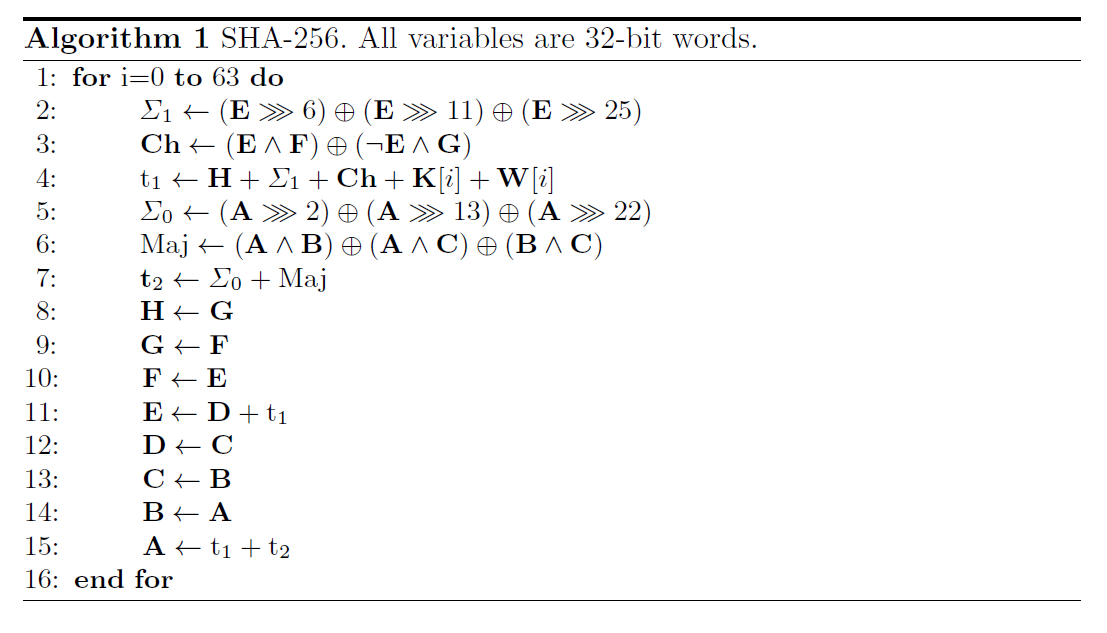
\includegraphics[width=0.8\textwidth]{./Images/quant-sha2-circ.png}
        \end{figure}
        Embedded images and charts in the section are from \cite{amy2016estimating}.
    \end{frame}

    \begin{frame}{SHA-256 Stretching}
        \begin{figure}[h]
            \centering
            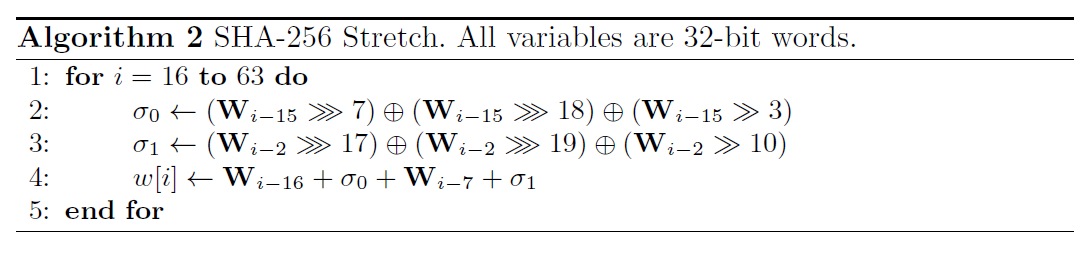
\includegraphics[width=0.8\textwidth]{./Images/quant-sha2-stretch.png}
        \end{figure}
        \begin{itemize}
            \item Both requires bitwise operations, bit shifting and addition
            \item Addition can be done by Ripple-Carry Adder
        \end{itemize}
    \end{frame}
    
    \begin{frame}{SHA-256 Quantum Circuit}
        \begin{figure}[h]
            \centering
            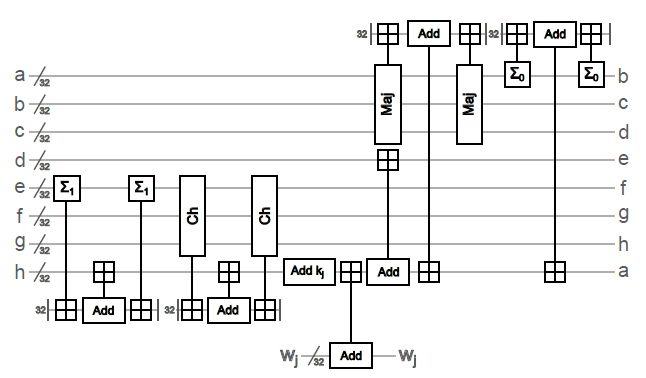
\includegraphics[width=0.7\textwidth]{./Images/quant-sha2-qcirc.png}
        \end{figure}
        \begin{itemize}
            \item Ignore padding and precalculations
            \item Thesis used 2402 qubits
            \item But with our calculation, 801 explicit qubits were sufficient
            \begin{itemize}
                \item 256 for hash, 32 $ \times $ 16 for $ w[i] $, 32+1 for ancilla
            \end{itemize}
        \end{itemize}
    \end{frame}
    
    \begin{frame}{SHA-256 Quantum Circuit Analysis}
        \begin{figure}[h]
            \centering
            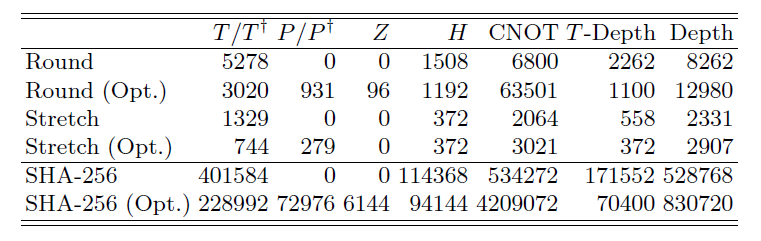
\includegraphics[width=0.7\textwidth]{./Images/quant-sha2-thesis-res.png}
        \end{figure}
        The literature has calculated the number of required gates.
        \begin{itemize}
            \item How to calculate these?
            \begin{itemize}
                \item Implement digital SHA-256 quantum circuit in OpenQASM\cite{cross2017open}
            \end{itemize}
            \item How to optimize these?
            \begin{itemize}
                \item T-par algorithm \cite{amy2014polynomial}
                \item Implemented in Feynman toolkit\footnote{\url{https://github.com/meamy/feynman}}
            \end{itemize}
        \end{itemize}
    \end{frame}
    
    \begin{frame}{Implementing SHA-256 in OpenQASM 2.0}
        OpenQASM : \textit{an imperative programming language for describing quantum circuits}
        \begin{itemize}
            \item Latest version : 3.0(Pre-release), 2.0
            \item Feynman accetps 2.0 format
            \item Problem: 2.0 lacks basic operations
            \begin{itemize}
                \item Only qubits/bits available, no loops, no array slicing
            \end{itemize}
        \end{itemize}
    \end{frame}
    
    \begin{frame}{Implementing SHA-256 in OpenQASM 2.0}
        \begin{minipage}[0.65\textheight]{\textwidth}
        \begin{columns}[T]
            \begin{column}{0.55\textwidth}
                \begin{figure}[t]
                    \centering
                    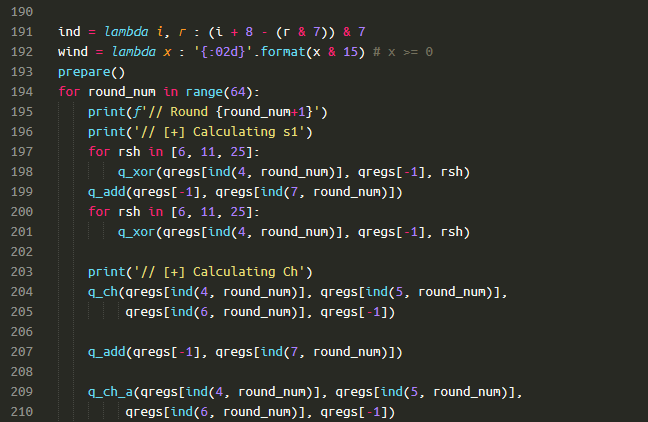
\includegraphics[width=\textwidth]{./Images/quant-sha2-py-code.png}
                \end{figure}
            \end{column}
            \begin{column}{0.45\textwidth}
                We made a code to generate SHA-256 OpenQASM code in Python 3.6.
                \begin{itemize}
                \item Excluding preambles like hardcoded gate definitions, 100 lines were sufficient.
                \end{itemize}
            \end{column}
        \end{columns}
        \end{minipage}
    \end{frame}    
    
    \begin{frame}{Optimizing SHA-256}
        Generated OpenQASM code is quite long (36k lines)
        \begin{itemize}
            \item Gate calculation was successful
            \item However, optimizing with T-par as a whole failed due to memory limit
            \item Workaround: Split code into 32-64 parts
        \end{itemize}
        Our experiment has two criteria: optimization algorithm and round per code.
        \begin{itemize}
            \item Algorithms: \texttt{tpar}\cite{amy2014polynomial} and \texttt{cnotmin}\cite{amy2018controlled}
            \item Code size : 1/2 round per code (64/32 parts)
        \end{itemize}
    \end{frame}    
    
    \begin{frame}{Results}
    
        \begin{table}[h]
        \small
        \begin{tabular}{lrrrrr}
            \hline \hline
            SHA-256 Type & $T$ & $H$ & $X$ & $CNOT$ & Misc. \\ \hline
            Literature, na\"ive & 401584 & 114368 & 0 & 534272 &  \\ \hline
            Ours, na\"ive & 351232 & 100352 & 1986 & 465088 &  \\
            Ours, T-Par, 1r & 343040 & 100352 & 10730 & 661376 & \begin{tabular}[c]{@{}r@{}}8192\\ $SWAP$\end{tabular} \\
            Ours, CNOTmin, 1r & 343040 & 100352 & 10730 & 381824 &  \\ \hline
            Ours, T-Par, 2r & 343040 & 100352 & 10730 & 664832 & \begin{tabular}[c]{@{}r@{}}8192\\ $SWAP$\end{tabular} \\
            Ours, CNOTmin, 2r & 343040 & 100352 & 10730 & 385280 &  \\ \hline
            Literature, T-Par & 228992 & 94144 & 0 & 4209072 & \begin{tabular}[c]{@{}r@{}}72976 $P$,\\ 6144 $Z$\end{tabular} \\ \hline \hline
        \end{tabular}
        \end{table}
        `1r' and `2r' denotes 1 round per code and 2 rounds per code, respectively.
    \end{frame}
    
    \begin{frame}{Analysis: Incomplete Business}
    	Three strange discrepancies...
    	\begin{itemize}
    		\item Gate differences of na\"ive ones
    		\item Smaller decrement of $T$-gate
    		\item Increased $CNOT$ gate when applied 2 rounds per code compared to 1 rounds of code
    	\end{itemize}
    \end{frame}
    
    \begin{frame}{Analysis: Na\"ive Gate Difference}
    	Why did the Na\"ive gate differ?
    	\begin{itemize}
    		\item Different way of implementation
    		\item Specifically, we utilized $X$-gates; the literature did not.
    		\begin{itemize}
    			\item The reason for non-utilization is unknown
    		\end{itemize}
    		\item The overall gate would have decreased due to the usage of $X$-gates, but its difference is too large.
    	\end{itemize}
    \end{frame}
  	
  	\begin{frame}{Analysis: $T$-gate and $CNOT$-gate Discrepancies}
  		Why did $T$-gate decrease less, even after considering the reduced gate count?
  		
  		In the 2r case, the number of $CNOT$ gates decreased less than 1r case. Why?
  		\begin{itemize}
  			\item Cannot be sure
  			\item Possibility 1: Our implementation of SHA is wrong
  			\item[$\Rightarrow$] Possible, since we couldn't test it, but even after we searched for incorrect result multiple times in the source and its generator, we couldn't find the error.
  			\item Possibility 2: The software we used is wrong or is only partially implemented
  			\item[$\Rightarrow$] Possible, and most probable due to the $CNOT$ gate discrepancy.
  		\end{itemize}
  	\end{frame}
\end{document}